\chapter{STG}
\label{ch:stg}

% Uvod: Imperativni vs funkcijski programski jeziki
Glede na paradigmo delimo programske jezike na imperativne in deklarativne. Imperativni jeziki, kot so npr. C, Rust, Python, \dots, iz vhodnih podatkov izračunajo rezultat s pomočjo stavkov, ki spreminjajo notranje stanje programa. Ukazi oziroma stavki podrobno opisujejo kako naj se program izvaja, in jih je zato nekoliko lažje prevesti v strojne ukaze, ki jih zna izvajati procesor. Pri deklarativnem programiranju pa je program podan kot višjenivojski opis želenega rezultata, ki ne opisuje dejanskega poteka programa. Med deklarativne jezike štejemo npr. SQL, katerega program je opis podatkov, ki jih želimo pridobiti in kako jih želimo manipulirati, ne da bi podrobno opisovali kako naj sistem izvede te operacije.

% Funkcijski programski jeziki
Med deklarativne programske jezike pa spadajo tudi funkcijski. Ti za osnovno operacijo nad podatki smatrajo čisto (angl. pure) funkcijo, tj. funkcijo, ki za izračun svoje vrednosti uporablja le vrednosti svojih argumentov, ne pa tudi drugega globalnega stanja. Prednost čistih funkcij je, da bodo enaki vhodi vedno vračali enake izhode, kar omogoča optimizacijo programa s pomočjo memoizacije. Osnovni primitiv je v takih jezikih funkcija, kar pomeni, da jih je mogoče prirediti v spremenljivke, jih uporabiti kot argumente in rezultate drugi funkcij. Čist funkcijski program lahko tako opišemo kot kompozicijo čistih funkcij, ki vhod preslikajo v izhod.

Poleg čistih funkcij je ena izmed ključnih značilnosti nekaterih funkcijskih jezikov tudi leni izračun (angl. lazy evaluation). Leni izračun je strategija računanja vrednosti izrazov, pri kateri se vrednost izraza ne izračuna takoj, ko je definiran, ampak šele, ko je njegova vrednost dejansko potrebna. Ta pristop je tesno povezan z deklarativno naravo funkcijskega programiranja in omogoča pisanje bolj modularne in učinkovite kode.

V poglavju se bomo podrobneje posvetili \textit{lenim} funkcijskim jezikom, podrobneje bomo definirali leni izračun, ter predstavili Haskell, jezik, ki temelji na čistih funkcijah in lenosti. Podrobneje bomo opisali potek prevajanja jezika v vmesni jezik imenovan STG in opisali delovanje abstraktnega STG stroja, ki ga zna izvajati.

\section{Leni izračun}
\label{sec:leni-izracun}

% Kaj je semantika, primerjava stroge in nestroge semantike
Semantika programskega jezika opisuje pravila in principe, ki določajo kako se programi izvajajo. Semantiko za izračun izrazov v grobem delimo na strogo (angl. strict) in nestrogo (angl. non-strict). Večina programskih jezikov pri računanju izrazov uporablja strogo semantiko, ki določa, da se izrazi izračunajo \textit{takoj, ko so definirani}. Nasprotno, nestroga semantika določa, da se izrazi izračunajo šele, ko so dejansko potrebni za nadaljnjo obdelavo, oziroma se sploh ne izračunajo, če niso potrebni.

% Prevladovanje stroge semantike
Večina današnjih programskih jezikov temelji na strogi semantiki. Mednje spadajo tako imperativni jeziki, kot so npr. C, Rust, Python, kot tudi funkcijski programski jeziki kot sta npr. Ocaml in Lisp. Jezikov, ki temeljijo na nestrogi semantiki je bistveno manj, med njimi npr. jeziki Haskell, Miranda in Clean.

% Primer
\begin{code-box}{haskell}{Haskell}
konjunkcija :: Bool -> Bool -> Bool
konjunkcija p q =
	case p of
		False -> False
		True -> q
\end{code-box}

Kot primer si oglejmo razliko pri evalvaciji izraza izraza \texttt{konjunkcija False ((1 / 0) == 0)}. Jeziki, ki temeljijo na strogi semantiki ob klicu funkcije najprej izračunajo vrednosti argumentov. Ker pride pri izračunu drugega argumenta do napake, se izvajanje programa tukaj ustavi. Pri jezikih z nestrogo semantiko pa se ob klicu funkcije ne izračunajo vrednosti argumentov, temveč se računanje izvede šele takrat, ko je vrednost dejansko potrebovana. Ker je prvi argument pri klicu funkcije \texttt{False}, funkcija drugega argumenta ne izračuna in tako je rezultat klica vrednost \texttt{False}.

% Formalizacija stroge in nestroge semantike
Če semantika jezika dopušča izračun vrednosti izraza, kljub temu, da njegovi podizrazi nimajo vrednosti, jo imenujemo za strogo semantiko. Bolj formalno lahko uvedemo vrednost $\bot$, ki jo imenujemo tudi dno (angl. bottom) in predstavlja vrednosti izrazov, katerim ni mogoče izračunati normalne oblike. Če izraza \textit{expr} ne moremo evalvirati, lahko tako zapišemo kar $\textbf{eval}(expr) = \bot$. Za funkcijo enega argumenta pravimo, da je \textit{stroga}, če velja naslednji pogoj.

$$ f \: \bot = \bot $$

Za stroge funkcije torej velja, da če se argument ne bo izračunal, se tudi rezultat klica funkcije z argumentom ne  bo evalviral. Če funkcija ni stroga, pravimo da je nestroga.

% Strogi izračun
Strogi izračun (angl. eager evaluation) je način implementacija stroge semantike, pri katerem so vrednosti argumentov izračunane pred klicem funkcije. Strogemu izračunu zato pravimo tudi \komentar{klic po vrednosti} (angl. call by value). Obratno, je leni izračun (angl. lazy evaluation) način implementacije nestroge semantike. Pri lenem izračunu izrazi niso izračunani kadar jih \textit{priredimo} spremenljivki, temveč je njihov izračun odložen na poznejši čas, kadar je vrednost izraza dejansko potrebovana. Ker se izračun izvaja po potrebi po vrednosti, to strategijo imenujemo izračun po potrebi (angl. call by need).

% Prednosti in slabosti
Ena izmed slabosti strogega izračuna je v tem, da klicana funkcija morebiti argumenta sploh ne potrebuje, kar pomeni, da se je ob klicu funkcije vrednost argumenta izračunala brez potrebe. Prednost strogega izračuna pa je v tem, da je izvajanje bolj predvidljivo, saj za razliko od lenega izračuna natančno vemo kdaj se bodo argumenti evalvirali. Prednost lenega izračuna pa leži v tem, da so argumenti evalvirani \textit{največ enkrat}. Če namreč argument v telesu funkcije ni nikoli uporabljen, potem tudi ne bo nikoli izračunan. Če pa je uporabljen, bo njegova vrednost izračunana \textit{enkrat} in memozirana v vseh preostalih uporabah. Slabost lenega izračuna pa je v tem, da ga je težje implementirati in da se navadno izvaja počasneje od jezikov s strogim izračunom.

% TODO: Reduction order - normal vs leftmost outmost

\subsubsection{Redukcija grafa}

% Razlika med imperativnimi in funkcijskimi jeziki - izvajanje
Zgodnejši programski jeziki so bili namenjeni neposrednemu upravljanju ra\-ču\-nal\-ni\-ka in so kot taki precej odražali delovanje računalniške arhitekture na kateri so se izvajali~\cite{10.1145/72551.72554}. Funkcijski programski jeziki omogočajo večji nivo abstrakcije, so bolj podobni matematični notaciji in posledično tudi bolj primerni za dokazovanje pravilnosti programov. Višji nivo abstrakcije pa pomeni, da jih je težje prevajati oziroma izvajati na današnji računalniški arhitekturi. Ena izmed ovir pri implementaciji lenega izračuna je učinkovito upravljanje z odloženimi izrazi (angl. thunks) in zagotavljanje, da se ti izrazi izračunajo le, ko so resnično potrebni.

% Kako implementiramo leni izračun?
Leni izračun najpogosteje implementiramo s pomočjo redukcije gra\-fa~\cite{peyton1987implementation, 10.1145/72551.72554}. Pri tej metodi prevajalnik na pomnilniku najprej sestavi abstraktno sintaksno drevo programa, kjer vozlišča predstavljajo aplikacije funkcij oziroma operacije nad podatki, njihova podvozlišča pa odvisnosti med njimi. V procesu \textit{redukcije}, se sintaksno drevo obdeluje z lokalnimi transformacijami, ki ga predelujejo, dokler ni dosežena končna oblika, tj. dokler ni izračunan rezultat programa. Pri tem se sintaksno drevo zaradi deljenja izrazov (angl. expression sharing) navadno spremeni v usmerjen graf.

Slika \ref{fig:redukcija-aplikacije-pred} prikazuje abstraktno sintaktično drevo izraza $(\lambda x \, . \, \textsc{not} \; x) \; \text{True}$. Aplikacija funkcij je predstavljena z vozliščem @, ki vsebuje dva podizraza: funkcijo, ki se bo izvedla in njen argument. V tem primeru je funkcija anonimni lambda izraz $(\lambda x \, . \, \textsc{not} \; x)$, ki sprejme en argument. Pri redukciji, se vse uporabe parametra $x$ zamenjajo z vrednostjo argumenta \texttt{True}. Slika \ref{fig:redukcija-aplikacije-po} prikazuje drevo po redukciji. Ker se je v funkciji argument $x$ pojavil le enkrat, je rezultat redukcije še vedno drevo.

\begin{figure*}[ht]
	\centering
	\begin{subfigure}[b]{0.45\textwidth}
		\centering
		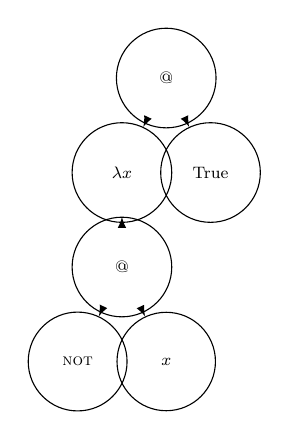
\begin{tikzpicture}[
			scale=0.75, transform shape,
			main/.style = {draw, circle},
			edge from parent/.style={draw,-latex},
			level distance=1.6cm,align=center,text width=0.75cm,
			]
			\node[main] (root) {@}
			child { node[main] {$\lambda x$}
				child { node[main] {@}
					child { node[main] {\textsc{not}} }
					child { node[main] {$x$} }
				}
			}
			child { node[main] {True} };
		\end{tikzpicture}
		\subcaption{Abstraktno sintaksno drevo \textit{pred} redukcijo}
		\label{fig:redukcija-aplikacije-pred}
	\end{subfigure}%
	\hfill
	\begin{subfigure}[b]{0.45\textwidth}
		\centering
		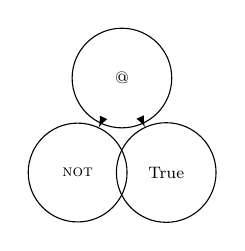
\begin{tikzpicture}[
			scale=0.75, transform shape,
			main/.style = {draw, circle},
			edge from parent/.style={draw,-latex},
			level distance=1.6cm,align=center,text width=0.75cm,
			]
			\node[main] (root) {@}
			child { node[main] {\textsc{not}} }
			child { node[main] {True} };
		\end{tikzpicture}
		\subcaption{Abstraktno sintaksno drevo \textit{po} redukciji}
		\label{fig:redukcija-aplikacije-po}
	\end{subfigure}
	\caption{Redukcija grafa izraza $(\lambda x \, . \, \textsc{not} \; x) \; \texttt{True}$}
	\label{fig:redukcija-aplikacije}
\end{figure*}

Slika \ref{fig:redukcija-dvojne-aplikacije} prikazuje en korak redukcije abstraktnega sintaksnega drevesa izraza $(\lambda x \, . \, \textsc{and} \; x \; x) \; (\textsc{not} \; \texttt{True})$. Po enem koraku redukcije sintaksnega telesa, se \textit{vse uporabe} parametra $x$ zamenjajo z njegovo vrednostjo. Ker je takih pojavitev več, pa rezultat ni več drevo, temveč acikličen usmerjen graf. Na pomnilniku tak izraz predstavimo z dvema kazalcema na isti objekt. Ko se objekt prvič izračuna, se vrednost objekta na pomnilniku posodobi z izračunano vrednostjo. Ob vseh nadaljnjih uporabah argumenta, tako ne bo potrebno še enkrat računati njegove vrednosti, s čemer dosežemo, da bo vsak argument izračunan največ enkrat. 

\begin{figure*}[ht]
	\centering
	\begin{subfigure}[b]{0.45\textwidth}
		\centering
		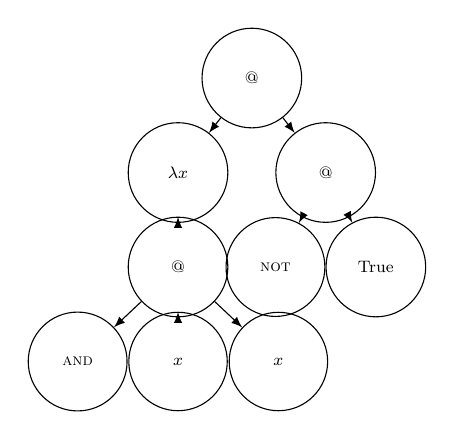
\begin{tikzpicture}[
			scale=0.75, transform shape,
			main/.style = {draw, circle},
			edge from parent/.style={draw,-latex},
			level distance=1.6cm,align=center,text width=0.75cm,
			level 1/.style={sibling distance=2.5cm},
			level 2/.style={sibling distance=1.7cm},
			]
			\node[main] (root) {@}
			child { node[main] {$\lambda x$}
				child { node[main] {@}
					child { node[main] {\textsc{and}} }
					child { node[main] {$x$} }
					child { node[main] {$x$} }
				}
			}
			child { node[main] {@}
				child { node[main] {\textsc{not}} }
				child { node[main] {True} }
			};
		\end{tikzpicture}
	\end{subfigure}%
	\hfill
	\begin{subfigure}[b]{0.45\textwidth}
		\centering
		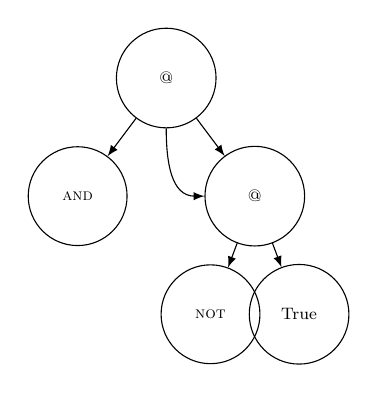
\begin{tikzpicture}[
			scale=0.75, transform shape,
			main/.style = {draw, circle},
			edge from parent/.style={draw,-latex},
			level distance=2cm,align=center,text width=0.75cm,
			]
			\node[main] (root) {@}
			child { node[main] {\textsc{and}} }
			child { edge from parent[draw=none] }
			child { node[main] (argument) {@}
				child { node[main] {\textsc{not}} }
				child { node[main] {True} }
			};
			\draw[-latex] (root) to[out=-90, in=180, looseness=1.1] (argument);
		\end{tikzpicture}
	\end{subfigure}
	\caption{Redukcija grafa izraza $(\lambda x \, . \, \textsc{and} \; x \; x) \; (\textsc{not} \; \texttt{True})$}
	\label{fig:redukcija-dvojne-aplikacije}
\end{figure*}

Slika \ref{fig:funkcija-y} prikazuje dve možni implementaciji ciklične funkcije $Y \; f = f \; (Y \; f)$. Za razliko od primerov na slikah \ref{fig:redukcija-aplikacije} in \ref{fig:redukcija-dvojne-aplikacije}, pri katerih je bilo reducirano sintaktično drevo še vedno usmerjen acikličen graf, pa temu pri funkciji $Y$ ni več tako. Funkcija $Y$ je namreč rekurzivna, kar pomeni, da se sama pojavi kot vrednost svojega argumenta. Na sliki \ref{fig:funkcija-y-kot-prosta-spremenljivka} je funkcija $Y$ implementirana s pomočjo acikličnega grafa, a v svojem telesu vseeno dostopa do proste spremenljivke $Y$, zaradi česar obstaja na pomnilniku cikel. Na sliki \ref{fig:funkcija-y-kot-cikel} je funkcija implementirana neposredno s pomnilniškem ciklu, kjer je vrednost argumenta kar vozlišče samo.

\begin{figure*}[ht]
	\centering
	\begin{subfigure}[b]{0.45\textwidth}
		\centering
		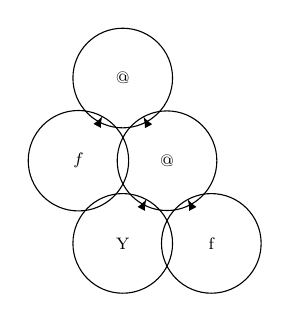
\begin{tikzpicture}[
			scale=0.75, transform shape,
			main/.style = {draw, circle},
			edge from parent/.style={draw,-latex},
			level distance=1.4cm,align=center,text width=0.75cm,
			]
			\node[main] (root) {@}
			child { node[main] {$f$} }
			child { node[main] {@}
				child { node[main] {Y} }
				child { node[main] {f} }
			};
		\end{tikzpicture}
		\subcaption{Funkcija $Y$ implementirana z uporabo proste spremenljivke}
		\label{fig:funkcija-y-kot-prosta-spremenljivka}
	\end{subfigure}%
	\hfill
	\begin{subfigure}[b]{0.45\textwidth}
		\centering
		\begin{tikzpicture}[
			scale=0.75, transform shape,
			main/.style = {draw, circle},
			edge from parent/.style={draw,-latex},
			level distance=1.4cm,align=center,text width=0.75cm,
			]
			\node[main] (root) {@}
			child { node[main] {$f$} }
			child { node (right) {} edge from parent[draw=none] };
			\coordinate [above=0.6cm of root] (above-root);
			\coordinate [right=0.4cm of right] (right-of-right);
			\coordinate (intermediate) at (right-of-right |- above-root);
			\draw[-latex] (root) -- (right.center) -- (right-of-right) -- (intermediate) -- (above-root) -- (root.north);
		\end{tikzpicture}
		\subcaption{Funkcija $Y$ implementirana kot cikličen usmerjen graf}
		\label{fig:funkcija-y-kot-cikel}
	\end{subfigure}
	\caption{Graf funkcije $Y \; f = f \; (Y \; f)$}
	\label{fig:funkcija-y}
\end{figure*}

\subsubsection{Zapis grafa na pomnilniku}

Leni izračun najpogosteje implementiramo s pomočjo zakasnitev (angl. thunks). Te so na pomnilniku predstavljene kot struktura s kazalcem na kodo, ki izračuna njihovo vrednost in polja, ki vsebujejo vezane in proste spremenljivke. Ob evalvaciji zakasnitve se najprej izračuna njihova vrednost, iz\-ra\-ču\-na\-no vrednost pa se shrani v strukturo na pomnilniku, da je ob naslednji evalvaciji ni potrebno ponovno računati. Pravimo, da se vrednost na pomnilniku posodobi. Na tak način se z nestrogo semantiko doseže, da se vsak izraz izračuna \textit{največ enkrat}. Če se argument ne pojavi nikjer v telesu funkcije, se zakasnitve nikoli ne računa, če pa se v telesu pojavi večkrat, se vrednost izračuna enkrat, za vsako nadaljnjo evalvacijo argumenta pa se preprosto vrne vrednost shranjeno na pomnilniku.

Slika \ref{fig:shema-vozlisca-pomnilnik} prikazuje eno izmed možnih predstavitev vozlišča grafa. Sestavljena je iz oznake vozlišča in polj z vsebino oziroma argumenti $a_1, \dots, a_n$. V poglavju \ref{sec:stg-jezik} bomo videli, da sta si struktura \ref{fig:shema-vozlisca-pomnilnik} in pomnilniški zapis objektov v jeziku STG precej podobna.

\begin{figure*}[ht]
	\centering
	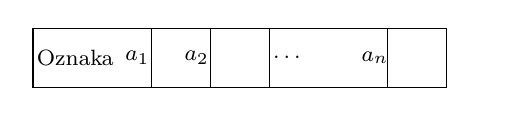
\begin{tikzpicture}[
		% Popravi vertikalno pozicioniranje teksta
		% https://tex.stackexchange.com/a/133237/324113
		verticalalign/.append style={font=\vphantom{Ag}},
		scale=0.75,
		]
		\draw[verticalalign] (0,0) rectangle ++(2,1) node[midway] {Oznaka};
		\draw[verticalalign] (2,0) rectangle ++(1,1) node[midway] {$a_1$};
		\draw[verticalalign] (3,0) rectangle ++(1,1) node[midway] {$a_2$};
		\draw[verticalalign] (4,0) rectangle ++(2,1) node[midway] {$\dots$};
		\draw[verticalalign] (6,0) rectangle ++(1,1) node[midway] {$a_n$};
	\end{tikzpicture}
	\caption{Pomnilniška predstavitev vozlišča grafa}
	\label{fig:shema-vozlisca-pomnilnik}
\end{figure*}

Slika \ref{fig:leni-izracun-pomnilnik-izraz} prikazuje predstavitev izraza $\textsc{and} \; (\textsc{not} \; \texttt{True}) \; (\textsc{not} \; \texttt{True})$ na pomnilniku. Celoten izraz je sestavljen iz dveh ovojnic, ki predstavljata dve aplikaciji. Spodnja ovojnica predstavlja izraz $\textsc{not} \; \texttt{True}$ in je sestavljena kot aplikacija funkcije \textsc{not} na argument z vrednostjo \texttt{0x0001}, tj. vrednost \texttt{True}. Zgornja ovojnica predstavlja aplikacijo funkcije \textsc{AND} na dva argumenta, ki sta predstavljena kot kazalca na drugo ovojnico. Ko se izraz $\textsc{not} \; \texttt{True}$ prvič izračuna, se ovojnica na pomnilniku posodobi z iz\-ra\-ču\-na\-no vrednostjo. Tako ob vseh nadaljnjih dostopih, vrednosti ni potrebno še enkrat računati, s čemer je dosežen ravno leni izračun.

\begin{figure*}[ht]
	\centering
	\begin{tikzpicture}[scale=0.8]
		\draw (0,0) rectangle ++(1,1) node[midway] {\textbf{@}};
		\draw (1,0) rectangle ++(2,1) node[midway] (and) {};
		\draw (3,0) rectangle ++(2,1) node[midway] (and-arg1) {};
		\draw (5,0) rectangle ++(2,1) node[midway] (and-arg2) {};
		
		\draw (0,-2) rectangle ++(1,1) node[midway] (app-not) {\textbf{@}};
		\draw (1,-2) rectangle ++(2,1) node[midway] (not) {};
		\draw (3,-2) rectangle ++(2,1) node[midway] {\texttt{0x0001}};
		
		\node (above-and) at (2,2) {\textsc{and}};
		\node (below-not) at (2,-3) {\textsc{not}};
		
		\draw[Circle-] (4,0.5) -- ++(0,-1);
		\draw[Circle-Latex] (6,0.5) -- ++(0,-1) -- ++(-7,0) -- ++(0,-1) -- ++(1,0);
		
		\draw[Circle-Latex] (2,0.5) -- ++(0,1);
		\draw[Circle-Latex] (2,-1.5) -- ++(0,-1);
		% \draw[-latex] (and) -- (above-and);
	\end{tikzpicture}
	\caption{Predstavitev izraza $\textsc{and} \; (\textsc{not} \; \texttt{True}) \; (\textsc{not} \; \texttt{True})$ na pomnilniku}
	\label{fig:leni-izracun-pomnilnik-izraz}
\end{figure*}

Ena izmed slabosti jezikov z lenim izračunom je, da je, za razliko od strogih imperativnih jezikov, zelo težko predvideti, koliko prostora bo program porabil. Prav tako je težko predvideti kdaj bodo vrednosti uporabljene in kdaj jih v programu ne potrebujemo več, zaradi česar vsi jeziki z lenim izračunom še vedno uporabljajo avtomatični čistilec pomnilnika.

% Povezava z naslednjim poglavjem
V nadaljevanju se bomo osredotočili na delovanje prevajalnika GHC (angl. Glasgow Haskell compiler), ki izvorno kodo napisano v programskem jeziku Haskell prevede v strojno kodo. Pri prevajanju se program transformira v več različnih vmesnih predstavitev (angl. intermediate representation), mi pa se bomo v magistrskem delu osredotočili predvsem na vmesno kodo imenovano STG jezik (angl. Spineless tagless G-Machine language), katerega delovanje bomo podrobneje opisali v razdelku \ref{sec:stg-jezik}.


\section{Prevajalnik GHC}
\label{sec:prevajalnik-ghc}

Prevajalnik GHC prevajanje iz izvorne kode v programskem jeziku Haskell v strojno kodo izvaja v več zaporednih fazah oziroma modulih. Vsaka faza kot vhod prejme izhod prejšnje, nad njim izvede določeno transformacijo in rezultat posreduje naslednji fazi. Faze glede na njihovo funkcijo v grobem delimo na tri dele. V prednjem delu (angl. front-end) se nad izvorno kodo najprej izvede leksikalna analiza, pri kateri se iz toka znakov, ki predstavljajo vhodni program pridobi abstraktno sintaktično drevo (angl. abstract syntax tree). Nad drevesom se izvede še zaporedje semantičnih analiz pri katerih se preveri ali je program pomensko pravilen. Sem sodi razreševanje imen, pri kateri se razreši vsa imena spremenljivk iz uvoženih modulov v programu in preveri ali so vse spremenljivke deklarirane pred njihovo uporabo. Izvede se še preverjanje tipov, kjer se za vsak izraz izpelje njegov najbolj splošen tip in preveri ali se vsi tipi v programu ujemajo.

\begin{figure}[h]
	\centering
	\begin{tikzpicture}
		\tikzset{
			every node/.append style={text width=1.4cm,execute at begin node=\setlength{\baselineskip}{1em},font=\footnotesize},
			block/.style={draw,rectangle,text width=2cm,align=center,minimum height=1cm,minimum width=2cm},
		}
		
		% Srednji del prevajalnika
		\node[block] (optimizacija) {Optimizacija};
		\node[coordinate, left=2.6cm of optimizacija] (center-levo) {};
		\node[coordinate, right=2.6cm of optimizacija] (center-desno) {};
		
		% Prednji del prevajalnika
		\node[block, above=0.55cm of center-levo] (semanticna-analiza) {Semantična analiza};
		\node[block, above=0.55cm of semanticna-analiza] (razclenjevanje) {Razčlen\-je\-van\-je};
		\node[block, below=0.55cm of semanticna-analiza] (izpeljava-tipov) {Izpeljava tipov};
		\node[block, below=0.55cm of izpeljava-tipov] (razsladenje) {Razsladenje};
		
		% Zadnji del prevajalnika
		\node[block, above=0.55cm of center-desno] (stg-to-cmm) {Izbira \texttt{C--} ukazov};
		\node[block, above=0.55cm of stg-to-cmm] (core-to-stg) {Izbira STG ukazov};
		
		% Moznosti prevajanja C-- -> strojna koda
		\node[block, minimum height=0.6cm, below=0.9cm of stg-to-cmm] (neposredno) {Neposredno};
		\node[block, minimum height=0.6cm, below=0.3cm of neposredno] (gcc) {GCC};
		\node[block, minimum height=0.6cm, below=0.3cm of gcc] (llvm) {LLVM};
		
		% 
		\node[coordinate, left=0.4cm of neposredno.west] (levo-od-neposredno) {};
		\node[coordinate, left=0.4cm of gcc.west] (levo-od-gcc) {};
		\node[coordinate, left=0.4cm of llvm.west] (levo-od-llvm) {};
		\draw[-] (levo-od-neposredno) -- (levo-od-gcc) -- (levo-od-llvm);
		\draw[->] (levo-od-neposredno) -- (neposredno);
		\draw[->] (levo-od-gcc) -- (gcc);
		\draw[->] (levo-od-llvm) -- (llvm);
		
		\node[coordinate, right=0.4cm of neposredno.east] (desno-od-neposredno) {};
		\node[coordinate, right=0.4cm of gcc.east] (desno-od-gcc) {};
		\node[coordinate, right=0.4cm of llvm.east] (desno-od-llvm) {};
		\draw[-] (desno-od-neposredno) -- (desno-od-gcc) -- (desno-od-llvm);
		\draw[-] (neposredno) -- (desno-od-neposredno);
		\draw[-] (gcc) -- (desno-od-gcc);
		\draw[-] (llvm) -- (desno-od-llvm);
		
		\node[coordinate, below=0.55cm of stg-to-cmm] (pod-stg-to-cmm) {};
		\node[coordinate] at (pod-stg-to-cmm -| levo-od-neposredno) (nad-levo-od-neposredno) {};
		\draw[-] (stg-to-cmm) -- (pod-stg-to-cmm) node[pos=0.5,right] {\scriptsize \texttt{C--}} -- (nad-levo-od-neposredno) -- (levo-od-neposredno) ;
		
		\draw[->] (razclenjevanje) -- (semanticna-analiza) node[pos=0.5,right] {\scriptsize AST};
		\draw[->] (semanticna-analiza) -- (izpeljava-tipov) node[pos=0.5,right] {\scriptsize AST};
		\draw[->] (izpeljava-tipov) -- (razsladenje) node[pos=0.5,right] {\scriptsize AST};
		
		\draw[->] (core-to-stg) -- (stg-to-cmm) node[pos=0.5,right] {\scriptsize STG};
		
		% Puscica "Generator vmesne kode" -> "Optimizacija vmesne kode"
		\node[coordinate, left=0.5cm of optimizacija.west] (levo-od-optimizacija) {};
		\node[coordinate] at (razsladenje -| levo-od-optimizacija) (desno-od-razsladenje) {};
		
		\draw[->] (razsladenje.east) -- (desno-od-razsladenje) -- (levo-od-optimizacija) node[pos=0.5,right] {\scriptsize Core} -- (optimizacija);
		
		% Puscica "Optimizacija vmesne kode" -> "Izbira ukazov"
		\node[coordinate, right=0.5cm of optimizacija.east] (desno-od-optimizacija) {};
		\node[coordinate] at (core-to-stg -| desno-od-optimizacija) (levo-od-izbira-ukazov) {};
		
		\draw[->] (optimizacija) -- (desno-od-optimizacija) -- (levo-od-izbira-ukazov) node[pos=1.0,left,align=right] {\scriptsize Core} -- (core-to-stg);
		
		% Vhodna povezava "Zacetek" -> "Leksikalna analiza"
		\node[coordinate, left=2cm of center-levo] (zacetek) {};
		\node[coordinate, left=0.5cm of razclenjevanje] (levo-od-razclenjevanje) {};
		\node[coordinate] at (zacetek -| levo-od-razclenjevanje) (desno-od-zacetek) {};
		
		\draw[->] (zacetek) -- (desno-od-zacetek) -- (levo-od-razclenjevanje) node[pos=0.2,left,text width=0.9cm] {\scriptsize tok\\znakov} -- (razclenjevanje);
		
		% Koncna povezava
		\node[coordinate, right=2cm of center-desno] (konec) {};
		\node[coordinate] at (konec -| desno-od-neposredno) (levo-od-konec) {};
		\draw[->] (desno-od-neposredno) -- (levo-od-konec) -- (konec) node[pos=1,above] {\scriptsize strojna\\koda};
		
		% Locevalne crte
		\node[coordinate, left=0.25cm of levo-od-optimizacija] (sprednji-del-center) {};
		\node[coordinate, above=3.7cm of sprednji-del-center] (sprednji-del-zgoraj) {};
		\node[coordinate, below=3.2cm of sprednji-del-center] (sprednji-del-spodaj) {};
		\draw[dashed] (sprednji-del-zgoraj) -- (sprednji-del-spodaj) node[pos=0,left=0.2cm,text width=2cm,align=right] {prednji del} node[pos=0,right=0.2cm,text width=2cm] {srednji del};
		
		\node[coordinate, right=0.25cm of desno-od-optimizacija] (zadnji-del-center) {};
		\node[coordinate, above=3.7cm of zadnji-del-center] (zadnji-del-zgoraj) {};
		\node[coordinate, below=3.2cm of zadnji-del-center] (zadnji-del-spodaj) {};
		\draw[dashed] (zadnji-del-zgoraj) -- (zadnji-del-spodaj) node[pos=0,right=0.2cm,text width=2cm] {zadnji del};
		
	\end{tikzpicture}
	\caption{Pomembnejše faze prevajalnika Glasgow Haskell compiler}
	\label{fig:shema-ghc}
\end{figure}

Bogata sintaksa programskega jezika Haskell predstavlja velik izziv za izdelavo prevajalnikov, saj zahteva natančno prevajanje raznolikih sintaktičnih struktur in konstruktov v strojno kodo. Težavo rešuje zadnji korak prednjega dela prevajalnika, imenovan \komentar{razsladenje} (angl. desugarification). V njem se sintaktično drevo jezika Haskell pretvori v drevo jezika Core, ki je minimalističen funkcijski jezik, osnovan na lambda računu. Kljub omejenemu naboru konstruktov omogoča Core zapis katerega koli Haskell programa. Vse nadaljnje faze prevajanja se tako izvajajo na tem precej manjšem jeziku, kar močno poenostavi celoten proces.

Srednji del (angl. middle-end) prevajalnika sestavlja zaporedje optimizacij, ki kot vhod sprejmejo program v Core jeziku in vrnejo izboljšan program v Core jeziku. Rezultat niza optimizacij se posreduje zadnjemu delu (angl. back-end) prevajalnika, ki poskrbi za prevajanje Core jezika v strojno kodo, ki se lahko neposredno izvaja na procesorju. Na tem mestu se Core jezik prevede v STG jezik, ta pa se nato prevede v programski jezik \texttt{C--}. Slednji je podmnožica programskega jezika C in ga je mogoče v strojno kodo prevesti na tri načine: neposredno ali z enim izmed prevajalnikov LLVM ali GCC. Prednost take vrste prevajanja je v večji prenosljivosti programov, saj znata LLVM in GCC generirati kodo za večino obstoječih procesorskih arhitektur, poleg tega pa imata vgrajene še optimizacije, ki pohitrijo delovanje izhodnega programa.

\section{STG jezik}
\label{sec:stg-jezik}

Kot smo si podrobneje pogledali v poglavju \ref{sec:leni-izracun}, lene funkcijske programske jezike najpogosteje implementiramo s pomočjo redukcije grafa. Eden izmed načinov za izvajanje redukcije je abstraktni STG stroj (angl. Spineless Tagless G-machine)~\cite{jones1992implementing, marlow2004making}, ki definira in zna izvajati majhen funkcijski programski jezik STG. STG stroj in jezik se uporabljata kot vmesni korak pri prevajanju najpopularnejšega lenega jezika Haskell v prevajalniku GHC (Glasgow Haskell Compiler)~\cite{GHC}.

% Kaj sploh je STG stroj in kaj je STG jezik

\subsection{Definicija jezika}
\label{sec:stg-definicija}

\komentar{Novejši članek~\cite{marlow2004making} pravi: "To make our discussion concrete we use a small, non-strict intermediate language similar to that used inside the Glasgow Haskell Compiler. / ... / In essence it is the STG language, but we have adjusted some of the details for this paper." Kako ustrezno napišemo, da se bomo v našem delu posvetili temu jeziku (in ne dejanskemu jeziku STG~\cite{jones1992implementing}), ker je nekoliko bolj preprost za razumevanje in ker nas ne zanimajo podrobnosti implementacije na dejanski računalniški arhitekturi?}

Sledi formalna definicija STG jezika. Pri tem bomo spremenljivke oz\-na\-če\-va\-li s poševnimi malimi tiskanimi črkami $x, y, f, g$, konstruktorje pa s poševnimi velikimi tiskanimi črkami $C$.
\begin{align*}
	literal \quad \coloneq& \quad \underline{int} \enspace \vert \enspace \underline{double} & \text{primitivne vrednosti}
\end{align*}

\komentar{Kakšen je prevod za boxed? Unboxed?}
STG jezik podpira dva primitivna (angl. unboxed) podatkovna tipa: celoštevilske vrednosti in števila s plavajočo vejico. Unboxed primitivne tipe označujemo s simbolom \komentar{lojtre}: \texttt{n\#}. Poleg tega jezik omogoča uvajanje novih algebraičnih podatkovnih tipov, ki jih lahko tvorimo oziroma inicializiramo s pomočjo konstruktorjev $C$. Pri tem je vredno omeniti, da so algebraični podatkovni tipi definirani v jeziku, ki ga prevajamo v STG, v našem primeru torej v Haskellu. Prav tako se v Haskellu izvaja tudi izpeljava in preverjanje tipov, abstraktni STG stroj pa med samim prevajanjem nima informacij o tipih.

\begin{align*}
	a, v \quad \coloneq& \quad literal \enspace \vert \enspace x & \text{argumenti so atomarni}
\end{align*}

Vsi argumenti pri aplikaciji funkcij in primitivnih operacij so v A-normalni obliki (angl. A-normal form)~\cite{flanagan1993essence}, kar pomeni, da so atomarni (angl. atomic). \komentar{Atomarni ali atomični argumenti?} Tako je vsak argument ali primitivni podatkovni tip ali pa spremenljivka. Pri prevajanju v STG jezik lahko prevajalnik sestavljene argumente funkcij priredi novim spremenljivkam z ovijanjem v \texttt{let} izraz in spremenljivke uporabi kot argumente pri klicu funkcije. Pri tem je potrebno zagotoviti, da so definirane spremenljivke unikatne oziroma, da se ne pojavijo v ovitem izrazu. Aplikacijo funkcije $f \; (\oplus \; x \; y)$ bi tako ovili v \texttt{let} izraz $\texttt{let} \enspace a = \oplus \; x \; y \enspace \texttt{in} \enspace f \enspace a$, s čemer bi zagotovili, da so vsi argumenti atomarni.

\begin{align*}
	k \quad \coloneq& \quad \bullet & \text{neznana mestnost funkcije}\\
	\vert& \quad n & \text{znana mestnost $n \geq 1$}\\
\end{align*}

Prevajalnik lahko med prevajanjem za določene funkcije določi njihovo mestnost (angl. arity), tj. število argumentov, ki jih funkcija sprejme. Ker pa je STG funkcijski jezik, lahko funkcije nastopajo tudi kot argumenti drugih funkcij, zato včasih določevanje mestnosti ni mogoče. V teh primerih funkcije označimo z neznano mestnostjo in jim med izvajanjem posvetimo posebno pozornost. Povsem veljavno bi bilo vse funkcije v programu označiti z neznano mestnostjo $\bullet$, a je mogoče s podatkom o mestnosti klice funkcij implementirati bolj učinkovito, zato se med prevajanjem izvaja tudi analiza mestnosti. 

\begin{align*}
	expr \quad \coloneq& \quad a & \text{atom}\\
	\vert& \quad f^k \: a_1 \dots a_n & \text{aplikacija funkcije ($n \geq 1$)}\\
	\vert& \quad \oplus \: a_1 \dots a_n & \text{primitivna operacija ($n \geq 1$)}\\
	\vert& \quad \texttt{let} \enspace x = obj \enspace \texttt{in} \enspace e & \text{} \\
	\vert& \quad \texttt{case} \enspace e \enspace \texttt{of} \enspace \{ alt_1; \dots; alt_n \}& \text{} \\
\end{align*}

Primitivne operacije so funkcije implementirane v izvajalnem okolju (angl. runtime) in so namenjene izvajanju računskih operacij nad \komentar{unboxed} primitivnimi podatki. Jezik podpira celoštevilske operacije \texttt{+\#}, \texttt{-\#}, \texttt{*\#}, \texttt{/\#}, in operacije nad števili s plavajočo vejico. Pri tem velja, da so vse primitivne operacije \textit{zasičene}, kar pomeni, da sprejmejo natanko toliko argumentov, kot je mestnost (angl. arity) funkcije. Če programski jezik omogoča delno aplikacijo primitivnih funkcij, potem je potrebno take delne aplikacije z $\eta$-dopolnjevanjem razširiti v nasičeno obliko. Pri tem delno aplikacijo ovijemo v nove lambda izraze z uvedbo novih spremenljivk, ki se ne pojavijo nikjer v izrazu. Tako npr. izraz \texttt{(+ 3)}, ki predstavlja delno aplikacijo vgrajene funkcije za seštevanje prevedemo v funkcijo $\lambda x . (+ 3 x)$ in s tem zadostimo pogoju zasičenosti.

Izraz \texttt{let} na kopici ustvari nov objekt in je kot tak tudi edini izraz, ki omogoča \komentar{alokacijo} podatkov na pomnilniku. Objekti na kopici bodo podrobneje opisani v nadaljevanju. V naši poenostavljeni različici STG jezika, izraz \texttt{let} ne omogoča rekurzivnih definicij. Edini vir rekurzije je v jeziku omogočen s pomočjo statičnih definicij (angl. top-level definitions), ki se lahko rekurzivno sklicujejo med sabo oziroma same nase.

\begin{align*}
	alt \quad \coloneq& \quad C \enspace x_1 \dots x_n \to expr & \text{algebraična alternativa}\\
	\vert& \quad x \to expr & \text{privzeta alternativa}\\
\end{align*}

Izraz \texttt{case} je sestavljen iz podizraza $e$, ki se evalvira in seznama alternativ $alts$, od katerih se vedno izvede \textit{natanko ena}. S preverjanjem tipov v fazi pred prevajanjem v STG je zagotovljeno, da vsi konstruktorji pri alternativah spadajo pod isti algebraični vsotni podatkovni tip (angl. sum type) in da so alternative izčrpne, tj. da obstaja privzeta alternativa ali da algebraične alternative pokrijejo ravno vse možne konstruktorje podatkovnega tipa. Izraz \texttt{case} najprej shrani vse žive spremenljivke, ki so uporabljene v izrazih v alternativah, na sklad doda \komentar{continuation} (angl. continuation), tj. naslov kjer se bo izvajanje nadaljevalo in nato začne računati vrednost izraza $e$. Zaradi bolj učinkovitega izvajanja, se pri prevajanju za konstruktorje vsotnih podatkovnih tipov generirajo oznake, navadno kar nenegativne celoštevilske vrednosti, ki se hranijo v objektu \textsc{con}. Pri razstavljanju sestavljenega podatkovnega tipa v \texttt{case} izrazu lahko tako primerjamo cela števila in ne celih nizov.

\begin{align*}
	obj \quad \coloneq& \quad \textsc{fun}(x_1 \dots x_n \to e) & \text{aplikacija}\\
	\vert& \quad \textsc{pap}(f \; a_1 \dots a_n) & \text{delna aplikacija}\\
	\vert& \quad \textsc{con}(C \; a_1 \dots a_n) & \text{konstruktor}\\
	\vert& \quad \textsc{thunk} \enspace e & \text{zakasnitev}\\
	\vert& \quad \textsc{blackhole} & \text{črna luknja}
\end{align*}

Kot smo že omenili, se novi objekti na kopici tvorijo le s pomočjo \texttt{let} izraza. Jezik STG podpira pet različnih vrst objektov, ki se razlikujejo glede na oznako v ovojnici na pomnilniku.

Objekt \textsc{fun} predstavlja funkcijsko ovojnico (angl. closure) z argumenti $x_1, \dots, x_n$ in telesom $e$, ki pa se lahko poleg argumentov $x_i$ sklicuje še na druge proste spremenljivke. Pri tem velja, da je lahko funkcija aplicirana na več kot $n$ ali manj kot $n$ argumentov, tj. je curryrana.
% Andrej Bauer pravi, da je to okej.
% https://x.com/andrejbauer/status/621602561368399872

Objekt \textsc{pap} predstavlja delno aplikacijo (angl. partial application) funkcije $f$ na argumente $x_1, \dots, x_n$. Pri tem je zagotovljeno, da bo $f$ objekt tipa \textsc{fun}, katerega mestnost bo \textit{vsaj} $n$.

Objekt \textsc{con} predstavlja nasičeno aplikacijo konstruktorja $C$ na argumente $a1, \dots a_n$. Pri tem je število argumentov, ki jih prejme konstruktor natančno enako številu parametrov, ki jih zahteva.

Objekt \textsc{thunk} predstavlja zakasnitev izraza $e$. Kadar se vrednost izraza uporabi, tj. kadar se izvede \texttt{case} izraz, se izračuna vrednost $e$, \textsc{thunk} objekt na kopici pa se nato posodobi s preusmeritvijo (angl. indirection) na vrednost $e$. Pri evalvaciji zakasnitve se objekt \textsc{thunk} na kopici zamenja z objektom \textsc{blackhole}, s čemer se preprečuje puščanje pomnilnika~\cite{jones1992tail} in neskončnih rekurzivnih struktur. Objekt \textsc{blackhole} se lahko pojavi le kot rezultat evalvacije zakasnitve, nikoli pa v vezavi v \texttt{let} izrazu.

\begin{align*}
	program \quad \coloneq& \quad f_1 = obj_1 \: ; \: \dots \: ; \: f_n = obj_n
\end{align*}

Program v jeziku STG je zaporedje vezav, ki priredijo STG objekte v spremenljivke.

\subsection{Operacijska semantika}

Operacijska semantika malih korakov bo opisana s pravili podanimi v obliki, ki jo prikazuje enačba \ref{eq:operacijska-semantika-oblika-pravil}. Pri tem z $e$ označujemo izraze (iz poglavja \ref{sec:stg-definicija}), oznaka $s$ predstavlja sklad \komentar{nadaljevanj} (angl. continuation), $H$ pa kopico.

\begin{equation}
	e_1; \, s_1; \, H_1  \;\; \Rightarrow  \;\; e_2; \, s_2; \, H_2
	\label{eq:operacijska-semantika-oblika-pravil}
\end{equation}

Na skladu $s$ hranimo nadaljevanja, ki stroju povedo, kaj storiti, ko bo trenutni izraz $e$ izračunan. Zapis $s = k : s'$ označuje sklad $s$, kjer je $k$ trenutni element na vrhu sklada, $s'$ pa predstavlja preostanek sklada pod njim. Nadaljevanja so lahko ene izmed naslednjih oblik:

\begin{align*}
	k \quad \coloneq& \quad \texttt{case} \; \bullet \; \texttt{of} \; \{ alt_1; \dots; alt_n \}\\
	\vert& \quad \textit{Upd} \; t \; \bullet\\
	\vert& \quad (\bullet \; a_1 \dots a_n)
\end{align*}

Nadaljevanje $\texttt{case} \; \bullet \; \texttt{of} \; \{ alt_1; \dots; alt_n \}$ izvede glede na trenutno vrednost $e$ natanko eno izmed alternativ $alt_1, \dots, alt_n$. Pri nadaljevanju $\textit{Upd} \; t \; \bullet$ se zakasnitev na naslovu $t$ posodobi z vrnjeno vrednostjo, tj. trenutnim izrazom $e$.  Zadnje nadaljevanje $(\bullet \; a_1 \dots a_n)$ pa uporabi vrnjeno funkcijo nad argumenti $a_1, \dots, a_n$. Sestavimo ga kadar je pri klicu funkcije argumentov preveč. Če vemo, da funkcija sprejme $n$ argumentov, pri aplikaciji pa je podanih $n + k$ argumentov, bo na sklad dodano nadaljevanje $(\bullet \; a_{n + 1 } \dots a_{ n + k })$ s $k$ argumenti.

Kopica $H$ je v operacijski semantiki predstavljena kot \komentar{slovar} (angl. map), ki spremenljivke slika v objekte na kopici. Oznaka $H[x]$ predstavlja dostop naslova $x$ na kopici $H$. Imena spremenljivk se torej v operacijski semantiki kar enačijo s pomnilniškimi naslovi. V dejanski implementaciji je kopica kar zaporeden kos pomnilnika, do katerega dostopamo preko pomnilniških naslovov, naloga prevajalnika pa je, da spremenljivkam dodeli pomnilniške naslove in s tem zagotovi pravilno preslikavo spremenljivk na objekte v pomnilniku. Prav tako je vsak objekt \textsc{fun}, \textsc{thunk}, \dots na kopici predstavljen kot funkcijska ovojnica, ki hrani naslove oziroma vrednosti prostih spremenljivk, ki se v njem pojavijo.

Omenimo še, da je pri pravilih operacijske semantike vrstni red pomemben, saj se pri izvajanju izvede prvo pravilo, ki ustreza trenutnemu stanju abstraktnega STG stroja.

\subsubsection{Dodeljevanje novih objektov na pomnilniku}

Pravilo \textsc{let} poda operacijsko semantiko \texttt{let} izraza. Ta na kopici ustvari nov objekt $obj$ in ga priredi novi unikatni spremenljivki $x'$, ki ni uporabljena nikjer v programu, kar ustreza alokaciji še neuporabljenega naslova na kopici. Zapis $e[x' / x]$ predstavlja izraz $e$, v katerem so vse proste spremenljivke $x$ zamenjane z vrednostjo $x'$. Pri \texttt{let} izrazu se torej najprej alocira nov objekt na pomnilniku, nato pa se izvede telo, v katerem so vse pojavitve spremenljivke $x$ zamenjane z novim pomnilniškim naslovom.

\begin{equation}
\infer[let]{
	\text{$x'$ je sveža spremenljivka}
}{
	\texttt{let} \enspace x = obj \enspace \texttt{in} \enspace e; \, s; \, H
}{
	e[x'/x]; \, s; \, H
}
\end{equation}

V pravi implementaciji je substitucija $e[x'/x]$ implementirana kot prepisovanje spremenljivke $x$ z kazalcem na objekt $x'$ v klicnem zapisu funkcije.

\subsubsection{Pogojna izbira s stavkom \texttt{case}}

V primeru, da je izraz, ki ga evalviramo v \texttt{case} izrazu (angl. scrutinee) pomnilniški naslov, ki kaže na konstruktor $C$, potem se izvede telo veje s konstruktorjem $C$, pri katerem se vrednosti parametrov $x_1, \dots x_n$ zamenjajo z argumenti $a_1, \dots, a_n$ (pravilo \textsc{casecon}).

\begin{equation}
	\linfer[casecon]{}{
		\texttt{case} \enspace v \enspace \texttt{of} \enspace \{ \dots; C \, x_1, \dots, x_n \to e; \dots \}; \, s; \, H[v \mapsto \textsc{con}(C \, a_1 \dots a_n)]
	}{
		e[a_1 / x_1 \dots a_n / x_n]; \, s; \, H
	}
\end{equation}

Če se noben izmed konstruktorjev v algebraičnih alternativah ne ujema s konstruktorjem na naslovu $v$, ali če je $v$ \komentar{literal}, potem se izvede privzeta alternativa (pravilo \textsc{caseany}). Pri tem se v telesu alternative parameter $x$ zamenja z $v$. V STG jeziku so vrednosti objekti \textsc{fun}, \textsc{pap} in \textsc{con}.

\begin{equation}
	\infer[caseany]{
		(\text{$v$ je \komentar{literal}}) \lor (\text{$H[v]$ je vrednost, ki ne ustreza nobeni drugi alternativi})
	}{
		\texttt{case} \enspace v \enspace \texttt{of} \enspace \{ \dots; x \to e \}; \, s; \, H
	}{
		e[v/x]; \, s; \, H
	}
\end{equation}

Pravilo \textsc{case} začne izračun \texttt{case} izraza. Najprej se začne računati izraz $e$, na sklad pa se potisne \komentar{nadaljevanje} case izraza, ki se bo izvedlo, ko se bo vrednost $e$ do konca izračunala.

\begin{equation}
	\infer[case]{}{
		\texttt{case} \enspace e \enspace \texttt{of} \enspace \{ \dots \}; \, s; \, H
	}{
		e; \, (\texttt{case} \; \bullet \; \texttt{of} \; \{ \dots \}) : s; \, H
	}
\end{equation}

Zadnje pravilo \textsc{ret} se izvede, ko se izraz v \texttt{case} izrazu do konca izračuna v \komentar{literal} ali kazalec na objekt na kopici. Glede na tip objekta na katerega kaže spremenljivka $v$, se bo nato izvedlo eno izmed pravil \textsc{casecon} ali \textsc{caseany}.

\begin{equation}
	\infer[ret]{
		(\text{$v$ je \komentar{literal}}) \lor (\text{$H[v]$ je vrednost})
	}{
		v; \, (\texttt{case} \; \bullet \; \texttt{of} \; \{ \dots \}) : s; \, H
	}{
		\texttt{case} \enspace v \enspace \texttt{of} \enspace \{ \dots \}; \, s; \, H
	}
\end{equation}

Pomembno je še omeniti, da se pri izvajanju nikoli ne brišejo vezave objektov na kopici. V primeru pravila \textsc{casecon}, se tako iz kopice ne izbriše vezava $v \mapsto \textsc{con}(C \, a_1 \dots a_n)$. Brisanje elementov iz kopice je implementirano s pomočjo avtomatičnega čistilca pomnilnika.

\subsubsection{Zakasnitve in njih posodobitve}

Pravili \textsc{thunk} in \textsc{update} sta namenjeni izračunu zakasnitev. Če je trenutni izraz ravno kazalec na zakasnitev, potem se na sklad doda nov posodobitveni okvir $\textit{Upd} \; t \; \bullet$, ki kaže na spremenljivko $x$, ki se bo po izračunu posodobila. Prav tako se na kopici objekt zamenja z \textsc{blackhole}. Če med izračunom vrednosti izraza $e$ abstraktni stroj ponovno naleti na spremenljivko $x$, lahko predpostavi, da program vsebuje cikel. Ker nobeno izmed pravil operacijske semantike na levi strani ne vsebuje objekta \textsc{blackhole}, se v primeru ciklov tako izračun zaustavi.

\begin{equation}	
\infer[thunk]{}{
	x; \, s; \, H[x \mapsto \textsc{thunk}(e)]
}{
	e; \, (\textit{Upd} \; t \; \bullet) : s; \, H[x \mapsto \textsc{blackhole}]
}
\end{equation}

Pri pravilu \textsc{update} se izvede posodobitev zakasnitve na kopici, pri čemer se spremenljivko $x$ preusmeri na objekt na katerega kaže spremenljivka $y$.

\begin{equation}
\infer[update]{
	\text{$H[y]$ je vrednost}
}{
	y; \, (\textit{Upd} \; x \; \bullet) : s; \, H
}{
	y; \, s; \, H[x \mapsto H[y]
}
\end{equation}

V dejanski implementaciji se pri posodobitvi na pomnilniku prejšnji ob\-je\-kt prepiše s preusmeritvijo (angl. indirection). To je objekt, ki je (podobno kot ostali objekti v STG jeziku glede na sliko \ref{fig:shema-stg-objekt}) sestavljen iz kazalca na metapodatke objekta in še enega dodatnega polja - kazalca na drug objekt. To pa tudi pomeni, da morajo imeti vsi objekti na kopici prostora vsaj za 2 kazalca (2 polji), saj bi sicer pri posodobitvi prišlo do prekoračitve kopice oziroma prepisovanja naslednjega objekta.

\subsubsection{Klici funkcij z znano mestnostjo}

Pri pravilu \textsc{knowncall} gre za uporabo funkcije z mestnostjo $n$ nad natanko $n$ argumenti. Izvede se telo funkcije, v katerem so vsi parametri zamenjani z vrednostmi argumentov, sklad in kopica pa ostajata nespremenjena.

\begin{equation}
	\linfer[knowncall]{}{
		f^n \, a_1 \dots a_n; \, s; \, H[f \mapsto \textsc{fun}(x_1 \dots x_n \to e)]
	}{
		e[a_1 / x_1 \dots a_n / x_n]; \, s; \, H
	}
\end{equation}

Pravilo \textsc{primop} je zelo podobno pravilu \textsc{knowncall}, le da se vrednost primitivne operacije izračuna neposredno v okolju za izvajanje. Ker so primitivne operacije po definiciji v STG jeziku vedno nasičene, zanje niso potrebna nobena dodatna pravila.

\begin{equation}
	\infer[primop]{
		a = \oplus \, a_1 \dots a_n
	}{
		\oplus \, a_1 \dots a_n; \, s; \, H
	}{
		a; \, s; \, H
	}
\end{equation}

Pri pravilih \textsc{knowncall} in \textsc{primop} gre za aplikacijo funkcije z znano mestnostjo $n$ na natanko $n$ argumentov. Kaj pa če argumentov ni dovolj ali pa jih je preveč? V primeru, da je argumentov premalo, gre za delno aplikacijo funkcije. Če pa je argumentov preveč, je potrebno funkcijo najprej aplicirati na ustrezno število argumentov. Ko se bo aplikacija do konca izvedla, bo rezultat funkcija, ki jo apliciramo na preostanek argumentov.

\subsubsection{Klici funkcij z neznano mestnostjo}

Pravilo \textsc{exact} je zelo podobno pravilu \textsc{knowncall}, le ga gre v tem primeru za funkcijo neznane mestnosti. V tem primeru je število argumentov shranjeno v tabeli metapodatkov objekta \textsc{fun} na kopici, kot bomo videli v poglavju \ref{sec:abstraktni-stg-stroj}.

\begin{equation}
	\linfer[exact]{}{
		f^\bullet \, a_1 \dots a_n ; \, s; \, H[f \mapsto \textsc{fun}(x_1 \dots x_n \to e)]
	}{
		e[a_1 / x_1 \dots a_n / x_n]; \, s; \, H
	}
\end{equation}

Pravili \textsc{callk} in \textsc{pap2} se ukvarjata z aplikacijami funkcij, pri katerih je število argumentov različno od njihove mestnosti. Če je število argumentov $m$ več kot parametrov $n$ (pravilo \textsc{callk}), potem se prvih $n$ argumentov porabi pri aplikaciji funkcije, vrednosti preostalih argumentov $a_{n + 1}, \dots, a_m$ pa se doda na sklad. Ko se aplikacija do konca izračuna, bo rezultat še ena funkcija, ki je uporabljena na preostalih argumentih (pravilo \textsc{retfun}). Če argumentov pri aplikaciji ni dovolj, se na kopici ustvari nov objekt \textsc{pap}, ki predstavlja delno aplikacijo.

\begin{equation}
	\linfer[callk]{
		m > n
	}{
		f^k \, a_1 \dots a_m ; \, s; \, H[f \mapsto \textsc{fun}(x_1 \dots x_n \to e)]
	}{
		e[a_1 / x_1 \dots a_n / x_n]; \, (\bullet \; a_{n + 1} \dots a_m) : s; \, H
	}
\end{equation}
\vspace{1em}
\begin{equation}
	\linfer[pap2]{
		m < n, \text{$p$ je sveža spremenljivka}
	}{
		f^k \, a_1 \dots a_m ; \, s; \, H[f \mapsto \textsc{fun}(x_1 \dots x_n \to e)]
	}{
		p; \, s; \, H[p \mapsto \textsc{pap}(f \, a_1 \dots a_m)]
	}
\end{equation}

Pravilo \textsc{tcall} pokrije možnost, da funkcija še ni izračunana, torej da je zakasnitev. V tem primeru se prične računanje zakasnitve $f$, obenem pa se na sklad doda nadaljevanje $(\bullet \; a_1 \dots a_m)$, ki bo sprožilo klic funkcije, ko bo vrednost zakasnitve do konca izračunana.

\begin{equation}
	\linfer[tcall]{}{
		f^\bullet \, a_1 \dots a_m ; \, s; \, H[f \mapsto \textsc{thunk}(e)]
	}{
		f; \, (\bullet \; a_1 \dots a_m) : s; \, H
	}
\end{equation}

Pri pravilu \textsc{pcall} gre za uporabo delne aplikacije nad preostankom argumentov. V tem primeru se funkcija $g$ uporabi nad vsemi $m$ argumenti. Ker je $g$ zaradi definicije v poglavju \ref{sec:stg-definicija} zagotovo funkcija, se bo v naslednjem koraku zagotovo zgodilo eno izmed pravil \textsc{exact}, \textsc{callk} ali \textsc{pap2}.

\begin{equation}
	\linfer[pcall]{}{
		f^k \, a_{n + 1} \dots a_m ; \, s; \, H[f \mapsto \textsc{pap}(g \, a_1 \dots a_n)]
	}{
		g^\bullet \, a_1 \dots a_n \, a_{n + 1} \dots a_m; \, s; \, H
	}
\end{equation}

Zadnje pravilo \textsc{retfun}, ki deluje na podoben način kot pravilo \textsc{ret} pri \texttt{case} izrazih. Kadar se izraz evalvira v kazalec, ki kaže na funkcijo \textsc{fun} ali delno aplikacijo \textsc{pap} in je na skladu nadaljevanje z argumenti, se ustrezno izvede aplikacija funkcije nad argumenti.

\begin{equation}
	\infer[retfun]{
		(\text{$H[f]$ je \textsc{fun}(\dots)}) \lor (\text{$H[f]$ je \textsc{pap}(\dots)})
	}{
		f; \, (\bullet \; a_1 \dots a_n) : s; \, H
	}{
		f^\bullet \, a_1 \dots a_n; \, s; \, H
	}
\end{equation}

V nadaljevanju bomo na kratko opisali delovanje abstraktnega STG stroja in predstavitev objektov na pomnilniku.

\subsection{Abstraktni STG stroj}
\label{sec:abstraktni-stg-stroj}

\komentar{To poglavje ni dokončano, ker nisem bil prepričan, ali sodi v magistrsko delo.}

Slika \ref{fig:shema-stg-objekt} prikazuje strukturo STG objektov na pomnilniku. Vsak objekt je sestavljen iz kazalca na tabelo metapodatkov in vsebine objekta, ki je sestavljena iz kazalcev na druge objekte ali literalov (angl. literals), tj. celih števil oziroma števil s plavajočo vejico. Različni objekti nosijo različno vsebino. Objekt $\textsc{con}(C \; a_1 \, \dots \, a_n)$ je npr. predstavljen s strukturo, ki ima na prvem mestu kazalec do metapodatkov objekta tipa CON, vsebina pa ima $n$ polj, z vrednostmi argumentov $a_1, \dots, a_n$ (ki so, kot smo videli v poglavju \ref{sec:stg-definicija} atomarne vrednosti, tj. kazalci ali literali). 

Tabela metapodatkov vsebuje dodatne informacije, ki jih potrebujemo pri izvajanju programa. Sestavlja jo kazalec na kodo, vrsta objekta, struktura objekta in dodatna polja, ki so specifična vrsti objekta. Kazalec na kodo kaže na kodo, ki se izvede pri evalvaciji objekta. Vrsta objekta je oznaka (npr. kar celoštevilska vrednost), ki razlikuje pet različnih vrst objektov (\textsc{thunk}, \textsc{fun}, \textsc{pap}, \textsc{con}, \textsc{blackhole}) med seboj. Struktura objekta vsebuje podatke o tem katera polja predstavljajo kazalce in katera polja dejanske vrednosti oziroma literale. V STG stroju se uporablja za avtomatično čiščenje pomnilnika, saj je pri tem v prvem koraku potrebno ugotoviti kateri objekti so živi, to pa sistem stori tako, da preko kazalcev obišče vse objekte. Vsak objekt vsebuje še dodatna polja, ki pa so odvisna od vrste objekta. Tako funkcija \textsc{fun} npr. vsebuje njeno mestnost, medtem ko hrani konstruktor \textsc{fun} njegovo oznako.

\begin{figure*}[ht]
	\centering
	\begin{tikzpicture}[y=-1cm,scale=0.9]
		\draw (0,0) rectangle ++(2,0.75) node[midway] (info-kazalec) {};
		\draw (2,0) rectangle ++(4,0.75) node[midway] {Vsebina};
		
		\draw (1.5,1.25) rectangle ++(4,0.75) node[midway] {Kazalec na kodo};
		\draw (1.5,2) rectangle ++(4,0.75) node[midway] {Vrsta objekta};
		\draw (1.5,2.75) rectangle ++(4,0.75) node[midway] {Struktura objekta};
		\draw (1.5,3.5) rectangle ++(4,1.5) node[midway,align=center,font=\linespread{0.8}\selectfont] {Polja specifična\\vrsti objekta};
		
		\node at (1.5+7,1.25+0.375) {Koda};
		
		\draw[{Circle}-Latex] (1,0.375) -- (1, 1.25+0.375) --(1.5, 1.25+0.375);
		\draw[{Circle}-Latex] (1.5+4-0.25,1.25+0.375) -- (1.5+6,1.25+0.375);
		\draw [decorate,decoration={brace,amplitude=8pt,mirror,raise=3em}]
		(1.5,1.25+0.375) -- (1.5,1.25+3.75-0.375) node[midway,xshift=-7em,align=center,font=\linespread{0.8}\selectfont]{Metapodatki\\objekta};
	\end{tikzpicture}
	\caption{Struktura STG objektov na pomnilniku}
	\label{fig:shema-stg-objekt}
\end{figure*}

% Obstajata dve različici, prva~\cite{jones1992implementing} je starejša in 

% V sledečem poglavju bomo podali formalno definicijo jezika STG definirano v \cite{marlow2004making}. Od originalne implementacije v \cite{jones1992implementing} se razlikuje po tem, da implementacija ni več brez oznak (angl. tagless), temveč nosi vsak objekt na kopici še dodatno polje z informacijo o njegovi vrsti. Ker je število tipov objektov majhno, se za oznako objekta navadno uporablja kar celoštevilčna vrednost. V originalni implementaciji so bili vsi objekti na kopici predstavljeni enotno, kar je pomenilo bolj kompaktno predstavitev podatkov v pomnilniku, prav tako pa STG stroju ni bilo treba preverjati vrste objektov ob vsakem klicu funkcije. Prednost ponovne uvedbe oznak pa je v tem, da STG stroju ni potrebno vzdrževati dveh ločenih skladov za argumente in vrednosti, kar pa tudi poenostavi delovanje čistilca pomnilnika.
% TODO: Citat

% Razlika med modeloma potisni / vstopi in izračunaj / apliciraj
%Nestrogo semantiko je moč implementirati na dva različna načina:
%
\begin{itemize}
	\itemsep 0em
	\item Model \textbf{potisni / vstopi} (angl. push / enter) najprej potisne vse argumente na sklad in nato \textit{vstopi} v funkcijo. Funkcija je odgovorna za preverjanje ali je na skladu dovolj argumentov. Če jih ni, potem mora sestaviti delno aplikacijo na kopici in končati izvajanje. Če pa je argumentov preveč, jih mora funkcija s sklada vzeti le ustrezno število, ostale argumente pa pustiti, saj jih bo uporabila naslednja funkcija, tj. funkcija v katero se bo evalviral trenutni izraz.
	\item Model \textbf{izračunaj / uporabi} (angl. eval / apply) klicatelj najprej evalvira funkcijo in jo nato aplicira na ustrezno število argumentov. Pri aplikaciji je potrebno zahtevano število argumentov funkcije pridobiti med izvajanjem programa iz funkcijske ovojnice.
\end{itemize}

Modela se razlikujeta glede na prelaganje odgovornosti za ... Pri modelu potisni / vstopi mora klicana funkcija preveriti ali je na skladu dovolj argumentov. Pri modelu izračunaj in apliciraj pa mora klicoča funkcija med izvajanjem pogledati v funkcijsko ovojnico in jo poklicati z ustreznim številom argumentov.

% Katero različico trenutno uporablja Haskell

Izkaže se, da je hitrejši model izračunaj / apliciraj~\cite{marlow2004making}, zato je ta model tudi uporabljen v Haskellovem prevajalniku GHC.

% Kaj se spremeni, če dodamo enega in drugega

\subsection{Primer}
\komentar{Manjka primer izvajanja manjšega programa v STG jeziku.}
